\section{Transition Graphs}

Transition graphs (TG) are similar to Finite Automata (FA), the distinction being that transition graphs can have blocks of inputs on one transition, and do not need to have garbage collection for unwanted inputs.

\subsection{Definition and example}
A Transition Graph is the collection of three things:
\begin{enumerate}
    \item A finite set of states, at least one of which is designated as the \textbf{start state}, and some (maybe none) of which are designated the \textbf{final states} or \textbf{accepting states}
    \item An \textbf{alphabet} \(\Sigma\) of input letters from which input strings are formed.
    \item A finite set of \textbf{transitions}(edge labels) that show how to go from some states to some others, based on reading specified substrings on input letters (possibly even the null string \(\Lambda\)).
\end{enumerate}
A \textbf{successful path} is a series of edges beginning at some start state and ending at a final state.
The concatenation of all the substrings that label the edges in the path is a word \textbf{accepted} by this machine. The set of words accepted is the \textbf{language} of the transition graph.

It is important to note that every FA is a TG but not every TG is an FA.

\begin{figure}[h!]
    \centering
    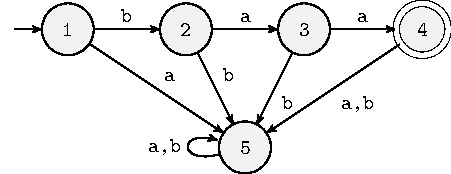
\includegraphics[width=0.7\linewidth]{lectures/figures/6-fa.pdf}
    \caption{Finite Automata accepting the language \(\{baa\}\).}
\end{figure}
\begin{figure}[h!]
    \centering
    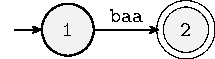
\includegraphics[width=0.33\linewidth]{lectures/figures/6-tg.pdf}
    \caption{Transition Graph accepting the language \(\{baa\}\).}
\end{figure}

On an FA it is not possible for any input to crash because there is always an outgoing edge for every possible letter from each state.
As long as there are unread letters, progress is possible.
TG's can crash when there is not an edge for the word to follow.


A TG in which some start state is also a final state will always accept the null string \(\Lambda\).

\subsection{Generalized Transition Graphs}

A generalized transition graph (GTG) is the collection of three things:
\begin{enumerate}
    \item A finite set of states, at least one of which is designated as the \textbf{start state}, and some (maybe none) of which are designated the \textbf{final states} or \textbf{accepting states}
    \item An \textbf{alphabet} \(\Sigma\) of input letters from which input strings are formed.
    \item A finite set of edges connecting some pairs of states, each labeled with a regular expression.
\end{enumerate}

\begin{figure}[h!]
    \centering
    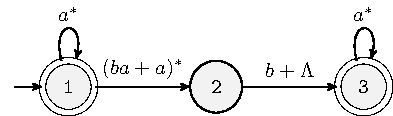
\includegraphics[width=0.5\linewidth]{lectures/figures/6-2gtg.pdf}
    \caption{Generalized Transition Graph of all words without two \(b\)'s in a row.}
\end{figure}

\subsection{Nondeterministic Finite Automata}
If there are multiple transitions that could be chosen simultaneously, the machine is considered \textbf{Nondeterministic}.
Human choices become a factor in selecting the path; the machine does not make all its own determinations.
\begin{figure}[h!]
    \centering
    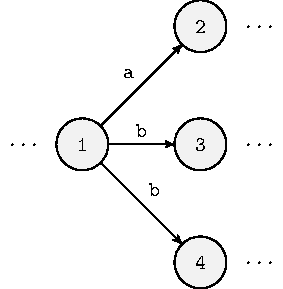
\includegraphics[width=0.4\linewidth]{lectures/figures/6-3nfa.pdf}
    \caption{Section of Nondeterministic finite automata.}
\end{figure}
